\section{Proposed Batch Bayesian Optimization Algorithm}

\begin{figure*}[tp!]
    \centering
    \subfigure[True phase margin curve, GP predictions, and Pareto set]{\label{fig:PF_example_1}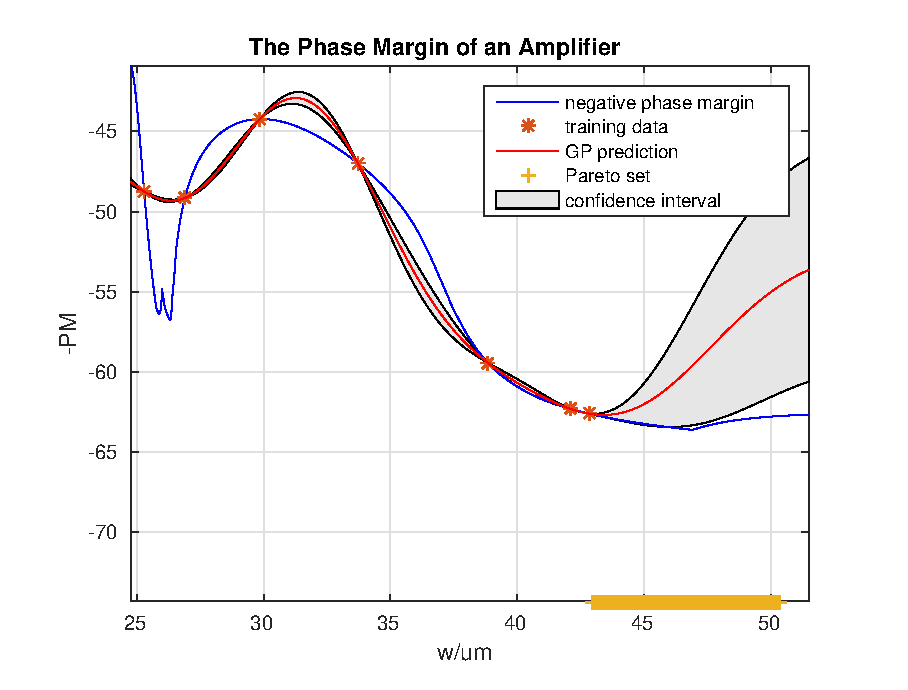
\includegraphics[width=0.49\textwidth]{./img/pm_gp_ps.eps}}
    ~
    \subfigure[The LCB, EI, and PI functions and the Pareto front]{\label{fig:PF_example_2}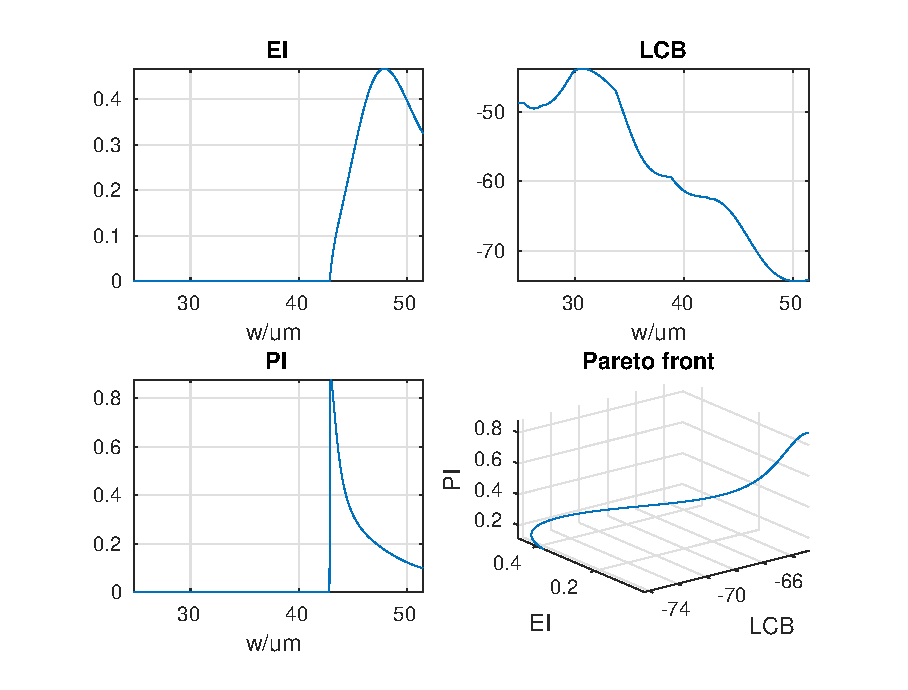
\includegraphics[width=0.49\textwidth]{./img/pf.eps}}
    \caption{Illustration of the multi-objective optimization of acquisition functions}
    \label{fig:PF_example}
        % \begin{subfigure}[]{width=0.5\textwidth}
        %     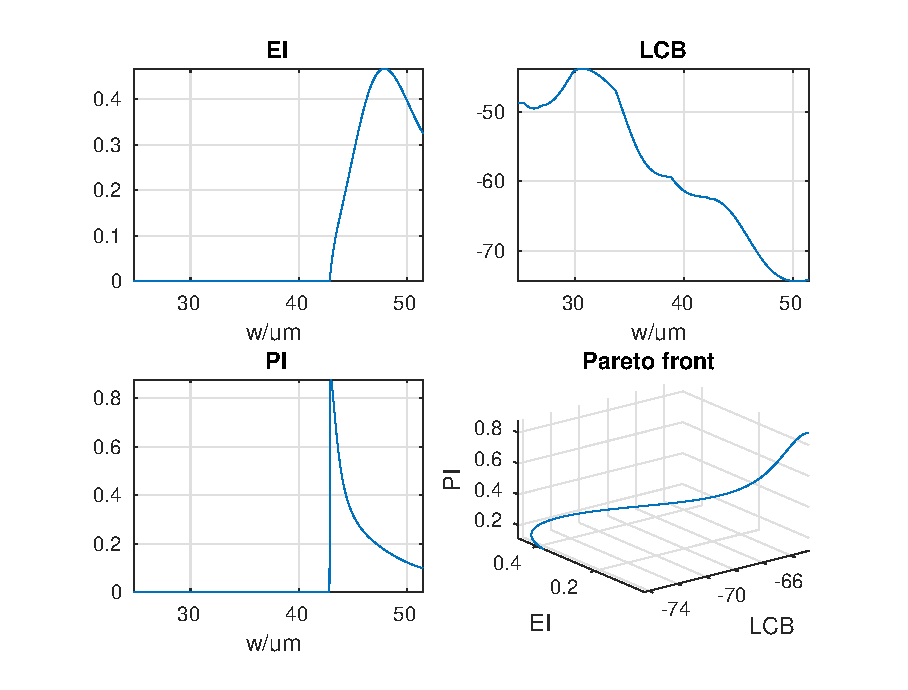
\includegraphics[width=0.5\textwidth]{./img/pf.eps}
        %     \caption{LCB, EI, PI and PF}
        %     \label{fig:PF_example_1}
        % \end{subfigure}
        % \begin{subfigure}[]{0.5\textwidth}
        %     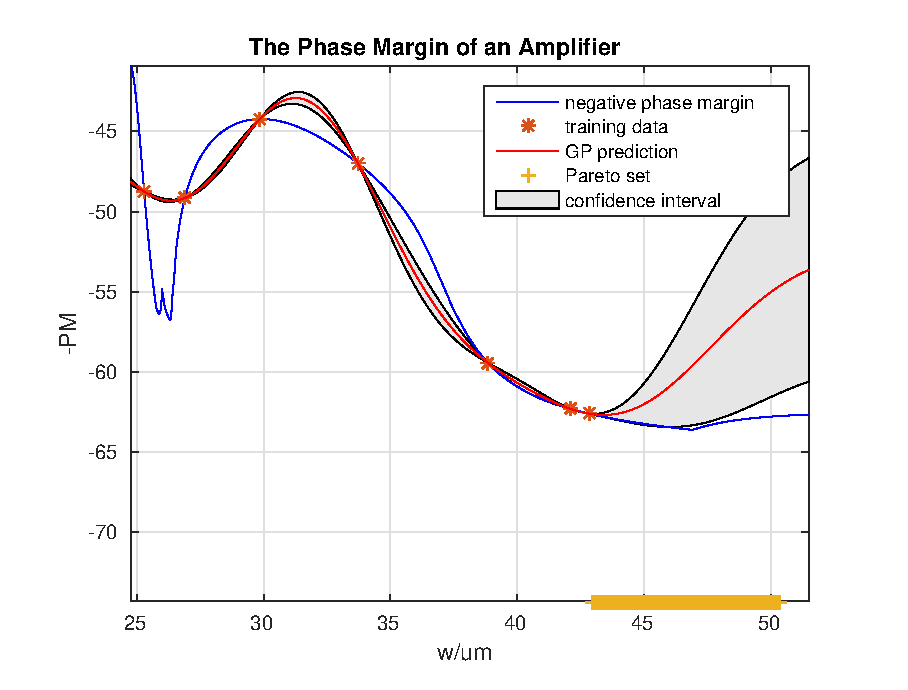
\includegraphics[width=0.5\textwidth]{./img/pm_gp_ps.eps}
        %     \caption{True curve, GP predictions and PS}
        %     \label{fig:PF_example_1}
        % \end{subfigure}
\end{figure*}

\subsection{Multi-objective Optimization of Acquisition Functions}\label{sec:MOForumlation}

\textcolor{red}{See how other MOBO paper formulate multi-objective optimization}

Unlike single-objective optimization, there are multiple objectives to optimize in multi-objective optimization problems\cite{MO_overview}, the multi-objective optimization problem is formulated as
\begin{equation}
    \label{eq:MOFormulation}
    \begin{aligned}
        & \text{minimize} & & f_1(\bm{x}),~\dots~,f_m(\bm{x}).
    \end{aligned}
\end{equation}
The multiple objectives to be optimizes can be conflicting, so that it is usually impossible to find a single solution that is the optimum of all objectives, the goal of multi-objective optimization algorithms is to approximate the \emph{Pareto front} of the objectives. A solution $\bm{x}_1$ is said to \emph{dominate} $\bm{x}_2$ if $\forall i \in \{1\dots m\},~f_i(\bm{x}_1) \le f_i(\bm{x}_2)$ and $\exists j \in \{1\dots m\}, f_j(\bm{x}_1) < f_j(\bm{x}_2)$. A design is \emph{Pareto-optimal} if it is not dominated by any other point in the design space and dominate at least one point. The whole set of the Pareto-optimal points in the design space is called the \emph{Pareto set}, and the set of Pareto-optimal points in the objective space is called the \emph{Pareto front}. It is often unlikely to get the whole Pareto front as there might be infinite points on the front, the goal of multi-objective optimization is to find a set of designs that approximates the true Pareto front.

There exist many mature multi-objective optimization algorithms, like the non-dominated sorting based genetic algorithm (NSGA-II)~\cite{nsgaii}, and the multi-objective evolutionary algorithm based on decomposition (MOEA/D)~\cite{moead}. In this paper, the multi-objective optimization based on differential evolution (DEMO)~\cite{demo} is used to solve multi-objective optimization problems, but other multi-objective optimization algorithms can also be applied.

\subsection{Batch Bayesian Optimization via Multi-objective Acquisition Ensemble}

Each acquisition function represents a unique selection strategy, different acquisition functions may not agree with each other about where to sample the next point. For example, the value of LCB function always decreases as the $\sigma(\bm{x})$ increases, however, for the PI function, when $\sigma(\bm{x})$ increases, the value of PI would decrease when $\mu(\bm{x}) < \tau$, and increase when $\mu(\bm{x}) > \tau$. For a noise-free problem, the EI values at already sampled points would always be lower than any unsampled location, while this property does not hold for the LCB function.


With multi-objective optimization, the best trade-off between acquisition functions can be captured by the Pareto front of these acquisition functions. We can then sample on the Pareto front to obtain multiple candidate points for the objective function evaluations. 

In the proposed MACE algorithm, the LCB, EI, and PI acquisition functions are selected, but other acquisition functions like KG and PES can also be incorporated into the MACE framework. In each iteration, the following MO problem is constructed:
\begin{equation}
    \label{eq:MO_LCB_EI_PI}
    \begin{aligned}
        & \text{minimize} & & \mathrm{LCB}(\bm{x}),~-\mathrm{EI}(\bm{x}),~-\mathrm{PI}(\bm{x}).
    \end{aligned}
\end{equation}
Then the DEMO multi-objective optimization algorithm is applied to solve the multi-objective problem in \eqref{eq:MO_LCB_EI_PI}. Once the Pareto front of LCB, EI and PI is obtained, the candidate evalution points are then randomly sampled from the Pareto front.

% TODO: We illustrate the proposed MACE algorithm using the Branin-Hoo function~\cite{dixon1978global}
% TODO: plot contour of Branin/Ei/LCB/PI, plot the PS and the PF
We illustrate the proposed MACE algorithm using an example of a real-world amplifier circuit. The optimization objective is to maximize the phase margin (PF) of the amplifier, so the FOM is defined as $\mathrm{FOM}(\bm{x}) = - \mathrm{PF}(\bm{x})$. The width of one of its transistor is the design variable, we sweep the width of the transistor and perform HSPICE simulations to get the FOM values. The curve of FOM values is plotted in Figure~\ref{fig:PF_example_1} (the blue line); several points are randomly sampled from the FOM curve to train the GP model, the LCB, EI, PI functions and the Pareto front of the acquisition functions are plotted in Figure~\ref{fig:PF_example_2}. We can see from Figure~\ref{fig:PF_example_2} that the optimal locations of the three acquisition functions are different, while their best trade-off is captured by the Pareto front. The Pareto set that represents the best trade-off between the three acquisition functions is the interval $[43, 50.4]$, as plotted in Figure~\ref{fig:PF_example_1}. The candidate points for the next batch of evaluations are randomly sampled from the Pareto set.

The proposed MACE algorithm is described in Algorithm~\ref{alg:MACE}.

\textcolor{red}{TODO: Input, Output parameters, see how other papers format the algorithm description}
\begin{algorithm}
\caption{Multi-objective Acquisition Ensemble Algorithm}
\label{alg:MACE}
\begin{algorithmic}[1]
\STATE Initial Sampling
\STATE Construct initial GP model
\FOR{t = 1, 2, \dots}
    \STATE Construct the LCB, EI and PI functions according to \eqref{eq:LCB} and \eqref{eq:PI_EI}
    \STATE Find the Pareto front of LCB, EI, PI function using the DEMO algorithm
    \STATE Randomly sample B points $\bm{x}_1, \dots, \bm{x}_B$ from the Pareto front where B is the batch size
    \STATE Evaluate $\bm{x}_1, \dots, \bm{x}_B$ to get $y_1 = f(\bm{x}_1),~\dots~,y_B = f(\bm{x}_B)$
    \STATE Update the GP model
\ENDFOR
\STATE Return best $f(\bm{x})$ recorded during iterations
\end{algorithmic}
\end{algorithm}

% \textcolor{red}{TODO: If there is space, discuss the approximation of EI in a new subsection "Implementation details"}
